\documentclass{thesisclass}
% Based on thesisclass.cls of Timo Rohrberg, 2009
% ----------------------------------------------------------------
% Thesis - Main document
% ----------------------------------------------------------------

\usepackage{caption}
\usepackage{blkarray}
\usepackage{framed}
\usepackage[linesnumbered,ruled]{algorithm2e}
\usepackage{multicol}
\usepackage{minted}
\usepackage{multicol}
\usepackage{wrapfig}
\usepackage{todonotes}
\usepackage{multirow}
\usepackage{multirow}
\usepackage{booktabs}
\usepackage{environ}
\usepackage{tabularx}
\usepackage[acronym,nomain]{glossaries}

%% ---------------------------------
%% | Information about the thesis  |
%% ---------------------------------

\newcommand{\myname}{Rudolf Biczok}
\newcommand{\mytitle}{Integration of internal and external gene expression and drug-perturbation data to empower novel immune therapies against Parkinson’s Disease}
\newcommand{\myinstitute}{Institute of Theoretical Computer Science}

\newcommand{\reviewerone}{Prof. Dr. Alexandros Stamatakis}
\newcommand{\reviewertwo}{Prof. Dr. Ralf Reussner}
\newcommand{\advisor}{Dr. Jitao David Zhang}

\newcommand{\timestart}{1st August 2018}
\newcommand{\timeend}{31st January 2019}

%% -------------------------------
%% |  Information for PDF file   |
%% -------------------------------

\hypersetup{
	pdfauthor={\myname},
	pdftitle={\mytitle},
	pdfsubject={Bioinformatics},
	pdfkeywords={Drug Discovery, Bioinformatics, Data Mining}
}

%% ---------------------------------
%% | Commands                      |
%% ---------------------------------

\newtheorem{definition}{Definition} \numberwithin{definition}{chapter}
\newtheorem{theorem}[definition]{Theorem}
\newtheorem{lemma}[definition]{Lemma}
\newtheorem{corollary}[definition]{Corollary}
\newtheorem{conjecture}[definition]{Conjecture}

\newcolumntype{C}{>{\centering\arraybackslash}X}

%% TODO : Is this ever used?
\NewEnviron{myTable}[4]{%
	\vspace{5px}%
	\centering%
	\rowcolors{2}{black!25}{white}%
	\captionsetup{type=table}
	\begin{tabular}{|#2|}%
		\arrayrulecolor{black}%
		\hline%
		\BODY
		\hline%
	\end{tabular}%
	\vspace{-6px}%
	\captionof{table}[#3]{#3#1} \label{#4}%
	\vspace{5px}
}

\NewEnviron{centeredFigure}[1][]{%
	\begin{figure}[#1]
		\centering
		\BODY
	\end{figure}	
}

\newcommand*\circled[1]{\tikz[baseline=(char.base)]{
		\node[shape=circle,draw,inner sep=2pt, fill=black] (char) {\textcolor{white}{#1}};}}

\newcommand{\thc}[1]{\textbf{\textcolor{white}{#1}}}

\newcommand{\myHeaderCell}[1]{\cellcolor{black}\thc{#1}}

\newcommand{\myMultiLineCell}[2][c]{%
	\begin{tabular}{@{}#1@{}}#2\end{tabular}%
}

\newcommand{\cbrac}[1]{\lbrace #1\rbrace}

%% --------------------------------
%% | Settings for word separation |
%% --------------------------------
% Help for separation:
% In german package the following hints are additionally available:
% "- = Additional separation
% "| = Suppress ligation and possible separation (e.g. Schaf"|fell)
% "~ = Hyphenation without separation (e.g. bergauf und "~ab)
% "= = Hyphenation with separation before and after
% "" = Separation without a hyphenation (e.g. und/""oder)

% Describe separation hints here:
\hyphenation{
% Pro-to-koll-in-stan-zen
% Ma-na-ge-ment  Netz-werk-ele-men-ten
% Netz-werk Netz-werk-re-ser-vie-rung
% Netz-werk-adap-ter Fein-ju-stier-ung
% Da-ten-strom-spe-zi-fi-ka-tion Pa-ket-rumpf
% Kon-troll-in-stanz
}

%Break links in URLs
\def\UrlBreaks{\do\/\do-}


%% ------------------------
%% |    Including files   |
%% ------------------------
% Only files listed here will be included!
% Userful command for partially translating the document (for bug-fixing e.g.)
\includeonly{
titlepage,
chapters/motivation,
chapters/introduction,
chapters/materials,
chapters/results,
chapters/conclusion,
chapters/appendix
}

% Generate the glossary
\makeglossaries

%%%%%%%%%%%%%%%%%%%%%%%%%%%%%%%%%
%% Here, main documents begins %%
%%%%%%%%%%%%%%%%%%%%%%%%%%%%%%%%%
\begin{document}

% Add common save boxes
\newsavebox{\saveBoxOne}
\newsavebox{\saveBoxTwo}
\newsavebox{\saveBoxThree}
\newsavebox{\saveBoxFour}
\newsavebox{\saveBoxFive}
\newsavebox{\saveBoxSix}
\newsavebox{\saveBoxSeven}
\newsavebox{\saveBoxEight}

% Remove the following line for German text
\selectlanguage{english}

\frontmatter
\pagenumbering{roman}
\include{titlepage}
\blankpage

%% -------------------------------
%% |   Statement of Authorship   |
%% -------------------------------

\thispagestyle{plain}

\vspace*{\fill}

\centerline{\textbf Statement of Authorship}

\vspace{0.25cm}

I hereby declare that this document has been composed by myself and describes my own work, unless otherwise acknowledged in the text.

\vspace{2.5cm}

\hspace{0.25cm} Heidelberg, 31st January 2019

\vspace{2cm}

\blankpage

%% -------------------
%% |   Abstract      |
%% -------------------

\thispagestyle{plain}

\begin{addmargin}{0.5cm}

\centerline{\textbf Abstract}

The primary objective of gene set enrichment analysis is to annotate a genes of interest with a-priory knowledge in the form of curated gene sets. The problem in this method lies in the large number of reported gene sets and their varying information content. Previous publications suggest to use unsupervised learning methods like hierarchical clustering or self-organized maps to increase interpretability, but there is no metric to assess the quality of these clustering methods or the difference between gene set itself. We therefore evaluated statistical methods (minkowski, jaccard, kappa-statistic), network-based methods (shortest path in protein-protein networks), and method based on natural language processing for their capability to measure a biologically plausible distance between gene sets. We used pathway trees from Reactome and a curated tree of immune cell types with corresponding gene sets to compare these distance methods.  \todo{TODO what is the conclusion?}

\vskip 2cm

\centerline{\textbf Deutsche Zusammenfassung}

%Kurze Inhaltsangabe auf deutsch.

\todo{Make german summary at the very end}

\vskip 2cm

\newpage

\centerline{\textbf Acknowledgements}

First and foremost I want to thank the two most valuable point of information Prof Dr. Alexandros Stamatakis and Dr. Jitao David Zhang. The open minded nature of Prof. Stamatakis made this research collaboration possible and his leading expertise in computational bioinformatics tremendously helped us to keep this master thesis in a academic format. Dr. Zhang also proved his courage and passion in academia by entrusting a theoretical biology research project to an computer science student. His knowledge as principle bioinformatician / biostatistician in an industrial and academic research environment complemented the methodical / computer science expertise of Stamatakis and me beyond expectations.

I send my greetings and thankfulness to Prof. Dr. Ralf H. Reussner, who did not hesitate to take the responsibility as second reviewer. I was a former participant in a two-term research project under the supervision of Prof. Reussner where he demonstrated a high level of methodical knowledge in the engineering aspect of computer science. 

In addition, I want to highlight the support from Gregor Sturm, Sarah Lutteropp, and Lucas Czech\todo{Will lucas be a Dr with the end of this thesis?}. Gregor Sturm is a former master thesis student of Dr. Zhang who shared the curated tree of immune cell types with their respective marker genes. He also eagerly helped me to extract  all necessary information from his publicly available code repository to save time on my side. Sarah Lutteropp is a PhD student of Prof. Stamatakis and shared her knowledge about methods and limitations in distance-based (phylogenetic) tree inference algorithms. Lucas Czech is also a PhD student under supervision of Prof. Stamatakis and provided me with an implementation skeleton for creating unsupervised clustering algorithms similar to $k$-means in C++.

Although I wish to thank every person in my live who inspired me, helped me, or even influenced my belief system, I must restrict myself to the following group of people that deserve a special place in this section: All members of the HITS Exelixis Lab (Prof. Dr. Alexandros Stamatakis, Dr. Alexey Kozlov, Lucas Czech, Sarah Lutteropp, Pierre Barbera, Benoit Morel, and Ben Bettisworth) and ROCHE BEDA group. Every single member treated me like an equal researcher.

I send my finally thanks and greetings to my parents, who are the only person on earth able to restrain my evil mind and my sister, who happened to be the younger sibling and by extension forced me to be a good role model.

\end{addmargin}

\blankpage

%% -------------------
%% |   Directories   |
%% -------------------

\tableofcontents
\listoftodos
\blankpage

%% -----------------
%% |   Main part   |
%% -----------------

\mainmatter
\pagenumbering{arabic}

%% ==============================
\chapter{Motivation}
\label{ch:motivation}
%% ==============================

\newacronym{rna}{RNA}{Ribonucleic Acid}
\newacronym{dna}{DNA}{Deoxyribonucleic Acid}
\newacronym{ppi}{PPI}{Protein Protein Interactions}

Molecular biology is the aspect of life science thats investigates biological processes on a cellular and molecular level. Biologists in this area seek answers for questions like: ``What is the structural and functional difference between neuron cells compared to other cell types in mammal species?'', ``What influence has chemical compound A when introduced to cell line C?'', or ``Is the cell line derived by following lab protocol A different from the cell line of protocol B?''.
%\begin{wrapfigure}{r}{0.4\textwidth}
%	\centering
%	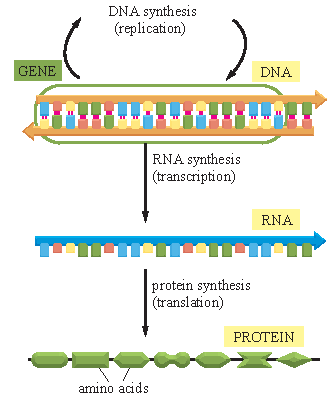
\includegraphics{figures/motivation/central_dogma.pdf}
%	\caption{Central dogma of molecular biology~\cite{citeulike:691434}}
%	\label{fig:central_docma}
%\end{wrapfigure}
%The biggest problem in answering this questions lies within the black-box nature of every living cell. We know that genes play an important role in determine the structure and basic behavior (also known as morphology) of every organism~\cite{citeulike:691434}. Ongoing research also reveals the functionalities behind each gene ofna n or    
The common procedure to research these questions is to conduct wet lab experiments on prepared cell cultures followed by a computer-assistant gene expression analysis. 
Gene expression is the fundamental biological process of every organism that describes the transcription of \acrfull{rna} from \acrfull{dna} and the translation from \acrshort{rna} to proteins~\cite{citeulike:691434}. 
Collecting and analyzing the gene expression level of every gene inside an organism allows us to identify differentially expressed genes that cause morphological differences between cell groups or cell types~\cite{doi:10.1093/bioinformatics/btp616}. To the end, bioinformaticians use public databases of gene sets to see which known cell components or biological processes are reflected by the previously inferred list of differential expressed genes. 
Every gene set represents discovered knowledge in form of name, description and involved genes of a particular biological process. 
Ideally, the entire procedure results in a list of gene sets that uniquely explain the effects of the original wet lab experiment~\cite{doi:10.1093/nar/gks461} (see \autoref{sec:gene_expression} for further information about gene expression analysis).

In reality, however, the information gain from reported gene sets is unsatisfying, because 
1) gene sets from even the same database source tend to have a high gene overlap, 
2) gene sets from publicly available databases can have many genes (>200), and 
3) gene set information like title and description can vary in quality depending on the source.
Existing literature suggest supervised clustering methods to organize gene sets into a more representative structure.  DAVID clustering, for instance, performs agglomerative clustering over pairwise kappa statistic between gene sets~\cite{Huang2007}. The authors of this algorithm claim that it maximizes the number of pairwise \acrfull{ppi} within each gene set cluster. They also, however, state that it is unclear if this optimization criterion is biologically justified. In general, there exist no gold standard to asses the biological similarity between two gene sets. Having such a gold standard for comparing gene sets on the other hand would make it possible to compare or even refine different clustering algorithm.

\section{Own contribution}

We present in this thesis a systematic evaluation of different categories of distance metrics for gene sets. We implemented metrics based on 1) statistic methods, 2) gene ontology trees, 3) protein-protein interaction networks, and 4) natural language processing methods. For comparing the performance of each distance implementation, we extracted gene sets from data sources whose relationships are already know and preserved as rooted trees. These data sources include X\todo{update to newest} subsets of the Reactome pathway database~\cite{doi:10.1093/nar/gki072} and a manually curated collection of marker genes for human immune cell types. We bundled all distances, data preprocessing and analysis scripts into a automated work flow that can be readily extended or included into other algorithms.

Besides gene set analysis, we also spend a significant amount of time building a client-server application with a web-based front-end for executing and storing gene expression analysis experiments. \todo{Ref}.

%% ==============================
\chapter{Introduction}
\label{ch:introduction}
%% ==============================

%A reader of the introduction should be able to answer the following questions, although not in any depth.
%
%    What is the thesis about?
%    Why is it relevant or important?
%    What are the issues or problems?
%    What is the proposed solution or approach?
%    What can one expect in the rest of the thesis?
%
%State what the thesis is about early. Don't keep the reader guessing until the end of the introduction, or worse, the end of the thesis (don't laugh, I have read draft theses that left me wondering after reading the entire document). You should provide a brief and gentle overview of the thesis topic (or problem) to give the reader enough context  to understand the rest of the introduction. Don't overwhelm the reader with detail at the start. You will provide the details later elsewhere in the thesis. Target the level of writing at one of your peers, but not necessarily somebody working in the same area.
%
%State why the topic is important. Address the "so what?" criteria. Why are you working on the topic? Why should somebody else be interested? Your motivation should be obvious after the introduction, but not necessarily provably so at this point.
%
%State what the major issues are in solving your problem. Coherently overview the issues in enough detail to be able to understand they exist, but don't go into details yet or attempt to prove they exist. The overview should be in just enough depth to understand why you might propose the your particular solution or approach you are taking.
%
%Describe your proposed solution or position you're taking. Again, you should not go into minute details, nor should you attempt to prove your solution at this point; the remainder of the thesis will describe and substantiate your solution in detail, that's what a thesis is :-)
%
%At this point the reader will know what you're working on, why, what are the major issues, and what your proposed solution is, but usually only if he takes your word for it. You should outline what the reader should expect in the rest of the thesis. This is not just the table of contents in sentence form, it is an overview of the remainder of the thesis so the reader knows what to expect. 
%
%
%--------------------------------
%

\section{Gene Expression Analysis} \label{sec:gene_expression}

\subsection{Gene set enrichment}

Even with the list of significant genes from a gene expression analysis, it is hard to impossible identifying the exact biological event that is the causal reason for the expression of these genes. The reason for this is the share amount of genes in higher species (e.g. homo sapiens has ~24,000 coding genes) whose actual functions is either unknown or highly ambiqous.

First, a biologist conducts experiments on prepared cell lines and then extracts RNA from these cells. 
Second, a bioinformatician utilize gene expression analysis pipelines to detect a list of  statistically significant gens within expression profiles. Finally, bioinformaticians use public databases of gene sets to see which cell components or biological processes are reflected by the previously inferred list of significant genes. 

\section{Protein-protein interactions}

\section{Gene ontology}

\section{Natural language processing}

%% ==============================
\chapter{Materials and methods}
\label{ch:methods}
%% ==============================

\section{Reference data}

\subsection{Reactome reference tree}

\subsection{Immune cell differentiation hierarchy}

\section{Distance measurements}

\subsection{Mathematical measurements}

\subsection{Network-based measurements}

\subsection{Word2vec models \& measurements}

%\section{Gene Expression Analysis}
%
%The most recurring task in pharmaceutical research \& early development is the gene expression analysis on a given date source. 
%
%\subsection{Methods for differential gene expression inferrence}
%
%Name | Strategy | Prefered Input Data
%-----|------------|--------------------
%[edgeR](http://doi.org/10.1093/bioinformatics/btp616) | Negative binomial distribution + Trimmed Mean of M values (TMM) Normalization | RNAseq
%[DEseq](https://doi.org/10.1186/s13059-014-0550-8) | Negative binomial distribution + scaling factor normalization procedure | RNAseq
%[limma](https://doi.org/10.1093/nar/gkv007) | Linear Modeling + voom transformation of counts (vor RNAseq) | RNAseq \& microarray
%
%The "rule of thumb" is to use limma for microarray data and edgeR for RNAseq data. DEseq is used to verify that a hypothesis based on edgeR results can also be derived from DEseq results (since edgeR is known to report more false positives).
%
%\subsection{Methods for batch-effect correction in meta-analysis}
%
%We use ComBat, SVA, and BioQC. Here we will probably have to compare different methods and reach a conclusion.
%
%\subsection{Methods for gene-set/pathway enrichment analysis}
%
%We use CAMERA, BioQC, and Fisher's exact test.
%Previously we found out that CAMERA and BioQC will lead to false negatives when many genes are differentially expressed, while Fisher's exact test will not (not published). We can verify this and make a meta-method to accommodate different scenarios.
%
%\section{ROGER}
%
%\subsection{ROGER Database}
%
%* **Annotations**
%* Gene Annotation (consumes biomart)
%* GeneAnnotation: Ensemble \& NCBI gen IDs. ROGER-internal GeneIndex, Gen meta data
%* Orthologs: Mapping between orthologous genes between different species
%* TranscriptioAnnotation: Ensemble Transcription ID and meta data
%* TranscriptRefSeq: NCBI Transcription ID and meta data
%* Genesets (consumes mongodb/json \& gmt)
%* DefaultGenesets: Available gen set data
%* DefaultGenesetCategory: For gen set categorization
%* DefaultGenesets2gene: Mapping of gen set data to gen annotations
%* **Input**
%* Datasets: Raw expression data
%* Phenodata
%* Designs: Relevant Feature matrix
%* Contrasts: Contrast matrix
%* **Methods \& Results**
%* GSEmethods: Used Gen enrichment method (e.g. CAMERA)
%* GSEtables: Gen enrichment results
%* DGEmethods: Used Differential Gen Expression inference method (e.g.  edgeR, limma)
%* DGEmodels: Used DGE model based on Desing and Cntrast information
%* DGEtables: Results from DEG inference
%
%\subsection{Annotation Problems}
%
%* Have to support both Ensembl and NCBI IDs
%* Ensembl has many unconsistent / deprecated data: Some Gene Symbols apper in multiple EnsembleGeneIds, 
%* Possible fix: pick the "most accurate on" (e.g. does it have a proper chromosone? Number of Transcripts etc.)
%
%% ![ROGER Schema](roger/old_schema.png)
%
%\subsection{RESTful APIs for scientific R pipelines}
%
%* [rplumber](https://www.rplumber.io/)
%* Fastest way to deploy REST services
%* Very low-level: No load balancing, no authentication, task management, ...
%* [OpenCPU](https://www.opencpu.org)
%* Load balancing
%* Lightwing WEB API basedn on JavaScript
%* No build-in support for [long running jobs]
%(https://github.com/opencpu/opencpu/issues/141)
%* No build-in task management
%* [Flask](http://flask.pocoo.org)
%* Python equivalent to OpenCPU
%* Established in the department
%* Requires wapper functions between python <-> R
%* No build-in task management
%
%\section{Differential Gene Expression}
%
%Lets assume we have a study consisting of a set of samples $D = \cbrac{A, B, C, D, E, F}$. Samples $A$ and $B$ are from macrophage cells, $C$ and $D$ are from microglia cells, and $E$ and $F$ are from monocyte cells. 
%
%Then we have basically two ground ways to model the experiments:
%
%\begin{lrbox}{\saveBoxOne}
%	\mintinline{R}{model.matrix(~CellType)} 
%\end{lrbox}
%
%\begin{lrbox}{\saveBoxTwo}
%	\mintinline{R}{model.matrix(~0+CellType)}
%\end{lrbox}
%
%\begin{lrbox}{\saveBoxThree}
%\begin{minipage}{5cm}
%	\[
%		\begin{blockarray}{cccc}
%			& \mu & \text{\rotatebox{90}{micro}} & \text{\rotatebox{90}{mono}} &  \\
%			\begin{block}{c(ccc)}
%				A & 1 & 0 & 0  \\
%				B & 1 & 0 & 0  \\
%				C & 1 & 1 & 0  \\
%				D & 1 & 1 & 0  \\
%				E & 1 & 0 & 1  \\
%				F & 1 & 0 & 1  \\
%			\end{block}
%		\end{blockarray}
%	\]
%\end{minipage}
%\end{lrbox}
%
%\begin{lrbox}{\saveBoxFour}
%\begin{minipage}{5cm}
%	\[
%		\begin{blockarray}{cccc}
%			& \text{\rotatebox{90}{macro}} & \text{\rotatebox{90}{micro}} & \text{\rotatebox{90}{mono}} &  \\
%			\begin{block}{c(ccc)}
%				A & 1 & 0 & 0  \\
%				B & 1 & 0 & 0  \\
%				C & 0 & 1 & 0  \\
%				D & 0 & 1 & 0  \\
%				E & 0 & 0 & 1  \\
%				F & 0 & 0 & 1  \\
%			\end{block}
%		\end{blockarray}
%	\]
%\end{minipage}
%\end{lrbox}
%
%\begin{lrbox}{\saveBoxFive}
%	\begin{minipage}{5.3cm}
%		\[ y \thicksim \mu + \beta_{\text{micro}} x_{\text{micro}} + \beta_{\text{mono}} x_{\text{mono}}\] 
%	\end{minipage}
%\end{lrbox}
%
%\begin{lrbox}{\saveBoxSix}
%	\begin{minipage}{5.3cm}
%		\[ \begin{split}
%		y \thicksim \ & \beta_{\text{macro}} x_{\text{macro}} + \beta_{\text{micro}} x_{\text{micro}} \\
%		& \beta_{\text{mono}} x_{\text{mono}}
%		\end{split} \]
%	\end{minipage}
%\end{lrbox}
%
%\begin{lrbox}{\saveBoxSeven}
%			\begin{minipage}{5.3cm}
%				\[
%					\begin{blockarray}{ccc}
%						\begin{block}{c(cc)}
%						\mu          & 0 & 0 \\
%						\text{micro} & 1 & 0 \\
%						\text{mono}  & 0 & 1 \\
%						\end{block}
%					\end{blockarray}
%				\]
%		\end{minipage}
%\end{lrbox}
%
%\begin{lrbox}{\saveBoxEight}
%	\begin{minipage}{5.3cm}
%			\[
%			\begin{blockarray}{cccc}
%			\begin{block}{c(ccc)}
%			\text{macro} & -1 & -1 & 0\\
%			\text{micro} & 1 & 0 & -1 \\
%			\text{mono}  & 0 & 1 & 1 \\
%			\end{block}
%			\end{blockarray}
%			\]
%	\end{minipage}
%\end{lrbox}
%
%\begin{table}[ht]
%
%	\begin{tabularx}{\linewidth}{|lCC|}%
%		\arrayrulecolor{black}%
%		\hline
%	
%		\rowcolor{black} & \thc{1 vs Average} & \thc{1 vs 1} \\
%	
%		\circled{1} & \usebox{\saveBoxOne} & \usebox{\saveBoxTwo} \\
%		\hline%
%	
%		\circled{2} & \usebox{\saveBoxThree} & \usebox{\saveBoxFour} \\
%		
%		\circled{3} & \usebox{\saveBoxFive} 
%		& \usebox{\saveBoxSix}  \\
%
%		\circled{4} & \usebox{\saveBoxSeven} 
%		& \usebox{\saveBoxEight}  \\
%		\hline%
%		
%		\hline
%	\end{tabularx}
%
%	\caption{Overview of example experiments} \label{fig:example_experiments}
%\end{table}
%
%\subsection{GO term enrichment}
%
%https://academic.oup.com/bioinformatics/article/22/13/1600/193669
%
%\subsection{GO term similarity}
%
%https://academic.oup.com/bioinformatics/article/26/7/976/213143

%% ==============================
\chapter{Results \& Discussion}
\label{ch:results}
%% ==============================

\section{Ground-truth comparison}

\section{Limitations}

%% ==================
\chapter{Conclusion}
\label{ch:conclusion}
%% ==================

%Recap on your thesis. It has been a long journey if the reader has made it this far. Remind the reader what the big picture was. Briefly outline your thesis, motivation, problem, and proposed solution.

%Now the most important part, draw conclusions based on your analysis. Did your proposed solution work? What are the strong points? What are the limitations?

%Significant issues identified in the thesis, or still outstanding after the thesis, should be describe as future work.

%% ----------------
%% |   Appendix   |
%% ----------------

\cleardoublepage

\appendix

%% ==============================
\chapter{Appendix}
\label{ch:appendix}
%% ==============================


\section{ROGER - Roche Omnibus of Gene Expression Regulation}

\subsection{State of the art}

\subsubsection{Transcriptomic data management}

\subsubsection{Differential Gene Expression Analysis}

\subsubsection{Gene Set Enrichment Analysis}

\subsection{Reimplementation}

\subsubsection{Data structures \& architecture}

\subsubsection{Visualizations \& data access}

\section{List of Acronyms}
%\setglossarysection{section}
\renewcommand{\glossarysection}[2][]{}
\printglossaries

\todo{List of figures?}
%\listoffigures

\todo{List of tables?}
%\listoftables

\normalsize

%% --------------------
%% |   Bibliography   |
%% --------------------

\cleardoublepage
\phantomsection
\addcontentsline{toc}{chapter}{\bibname}

\iflanguage{english}
{\bibliographystyle{alpha}}
{\bibliographystyle{babalpha-fl}} % german style

\bibliography{references}

\end{document}
